In this chapter we describe the experimental platform in which the measurements were carried out (Ref. \cite{zenesini2024false}) and we will then proceed with the FFT and ACF data analysis. The code for the analysis was written in the \textbf{\texttt{Python}} programming language.

\section{Experimental platform}
The experimental platform is composed of a bosonic gas of $^{23}$Na atoms, optically trapped and cooled below the condensation temperature. The initial spin state in which the system is prepared is $\ket{F, m_F} = \ket{2, -2} = \ket{\uparrow}$, with $F$ being the total angular momentum of the atom 
% ($\mathbf{F} = \mathbf{I} + \mathbf{J}$, takes into account the nuclear spin and the total angular momentum of the electrons) 
and $m_F$ its projection on the quantization axis. The $\ket{\uparrow}$ state is then coupled to $\ket{1, -1} = \ket{\downarrow}$ through microwave radiation with amplitude $\Omega_R$. The relevant scattering lengths concerning the two states are $a_\uparrow = 64.3 a_0$, $a_\downarrow = 54.5 a_0$ and $a_{\uparrow\downarrow} = 64.3 a_0$.

The trapping potential is harmonic in all three directions, but strongly asymmetric concerning the radial ($\rho$) and axial ($x$) directions. In fact, the trapping frequencies are respectively $\nu_\rho = 2\ \unit{\kilo\hertz}$ and $\nu_x = 20\ \unit{\hertz}$, yielding an elongated system (cigar-shaped) with inhomogeneous density. The spatial size of the system is given by the Thomas-Fermi radii $R_\rho = 2\ \unit{\micro\meter}$ and $R_x = 200\ \unit{\micro\meter}$, calculated with Eq.\ \eqref{eq:TF}. This particular setup is helpful for suppressing the radial spin dynamics of the condensate and thus reducing it from a 3D system of density $n_{3D}(r_\perp,x)$ to a 1D system of linear density $n(x)$, with the only difference being the renormalization of the interaction constant
\[
    \delta g \to k = \frac{2}{3}\frac{n_{3D}}{n}\delta g\, .
\]

In order to extract the density distribution, the two spin states are treated independently one from another, and a spin-selective imaging process is performed. Then, an integration along the transverse direction is carried out, obtaining two 1D density profiles $n_\uparrow(x)$ and $n_\downarrow(x)$, from which one can extract the relative magnetization
\begin{equation}
    Z(x) = \frac{n_\uparrow(x) - n_\downarrow(x)}{n_\uparrow(x) + n_\downarrow(x)}\, .
    \label{eq:magnetization}
\end{equation}
Due to the quantum nature of the system, once imaged the condensate loses its spatial information and it has to be prepared back in the initial state, allowing for another measurement.

% It is possible to study the two-component system by separating the treatment on the density ($n = n_\uparrow + n_\downarrow$) and the spin ($nZ = n_\uparrow - n_\downarrow$) degrees of of freedom. 
% While the density is described by a continuity equation, the spin behaviour is ruled by a magnetic mean-field Hamiltionian, that presents a first-order phase transition in the central region of the system when $\Omega_R < |k|n$, where $k \propto \Delta a$. At fixed values of $\Omega_R$, the experiment can be tuned by the parameter $\delta$, expressing the \textit{detuning}. In general, the mean-field energy landscape $E(Z)$ is described by an asymmetric double-well, that becomes symmetric for $\delta = 0$. In the case of $\delta < 0$, the energy is minimized by negative values of $Z$. 

\section{Raw data}
Raw data is organized in a hierarchical system. At a fixed instant, the condensate's measured data are called a \textit{shot} (it refers to the imaging process). Each shot is part of a series of them that can be analyzed as the time evolution of a single system: this series is called a \textit{sequence}. Eventually, during a \textit{day} of measurements, many sequences may be collected, and a selection of them will be studied in the following analysis. For each sequence, the experimental data contains also the radiation coupling $\Omega_R$ in a range between $2\pi \times 200$ \unit{\hertz} and $2\pi \times 800$ \unit{\hertz} (it changes from one day of measurements to another) and the detuning $\delta$ in a range between $2\pi \times 100$ \unit{\hertz} and $2\pi \times 600$ \unit{\hertz}. For each shot, the experimental waiting time $t$ is saved and it provides information on the time interval passed before the imaging process, ranging from 1 \unit{\milli\second} to 300 \unit{\milli\second}. 

A shot contains all the information on the system after waiting for a time $t$, including the two population densities, $n_\uparrow(x)$ for to the atoms in the state $\ket{\uparrow}$ and $n_\downarrow(x)$ for the atoms in the state $\ket{\downarrow}$, distributed on a length scale from 0 to 400 pixels. The spatial resolution of the image is $1\ \text{pixel} = 1.025\ \unit{\micro\meter} \approx 1\ \unit{\micro\meter}$, so the two length units will often be used interchangeably. The magnetization data $Z(x)$ is calculated with Eq.\ \eqref{eq:magnetization} and, by definition, composed of a series of values ranging from $-1$ (all atoms in the state $\ket{\downarrow}$) to $1$ (all atoms in the state $\ket{\uparrow}$).

% Our focus here is to study the magnetization of the system, developing a method to analyze the effects of its bubble formation, and then proceed with the density behaviour.
Our focus here is to characterize the bubble properties in relation to $\Omega_R$, $\delta$, $t$ by utilizing the magnetization of the system. First, we need to extract the spatial parameters of the bubble in order to locate it in each shot, then we will proceed with the study of its evolution.

\subsection{Bubble fit parameters}
In order to localize the bubble in a shot, the most interesting parameters to retrieve are the bubble center $x_0$ and its width $\sigma_B$.
However, not all shots contain a bubble, namely the ones taken when the bubble was not formed yet. We can easily classify the two types of shots by computing the magnetization average in the central region and using a threshold value, set to $Z_{\rm thr} = -0.2$. 
% The no-bubble shots will be useful later, when dealing with the noise frequency spectrum.

\begin{figure}[h!]
    \centering
    \includegraphics[width = 0.75\textwidth]{figures/chap2/arctan_fit.png}
    \caption{Example of fit results performed on a shot. First, the data is fitted with the double-arctangent function of Eq.\ \eqref{eq:double-atan}, then each shoulder is fitted with a single-arctangent, namely the one of Eq.\ \eqref{eq:atan}. This ensures a better estimation of the shoulder centers and thus of the bubble width. Eventually, a last fit is done with the piecewise function of Eq.\ \eqref{eq:fit_exp}, in order to capture the inside/outside discontinuity and the exponential tails.}
    \label{fig:atan-fit}
\end{figure}

To parametrize the bubble, the magnetization data is fitted with a double-arctangent function
\begin{equation}
    Z_{\rm fit}(x) = -A \left[\frac{2}{\pi}\arctan(\frac{x-c_1}{w_1}) - \frac{2}{\pi}\arctan(\frac{x-c_2}{w_2})\right] + \Delta\, ,
    \label{eq:double-atan}
\end{equation}
where $c_1$ and $c_2$ are the centers' positions of the arctangent "shoulders", and $w_1$ and $w_2$ are their characteristic widths. 
% \begin{figure}[h!]
%     \centering
%     \begin{minipage}[t]{0.47 \textwidth}
%         \centering
%         \includegraphics[width = \linewidth]{figures/chap2/arctan_fit.png}
%         \caption{Example of double arctangent and piecewise exponential fit results performed on a shot.}
%         \label{fig:atan-fit}
%     \end{minipage}
%     \hspace{0.02\textwidth}
%     \begin{minipage}[t]{0.47 \textwidth}
%         \centering
%         \includegraphics[width = \linewidth]{figures/chap2/gaussian_fit.png}
%         \caption{Example of gaussian fit results performed on a shot where the double arctangent fit procedure fails.}
%         \label{fig:gaussian-fit}
%     \end{minipage}
% \end{figure}
Then, for a better result, a further fit is performed on each shoulder with a single-arctangent function
\begin{equation}
    Z_{\rm fit}(x) = -A \frac{2}{\pi}\arctan(\frac{x-c_{1,2}}{w_{1,2}}) + \Delta\, ,
    \label{eq:atan}
\end{equation}
yielding the shoulder center position $c_{1,2}$. Eventually, we obtain the bubble center position $x_0 = (c_1 + c_2)/2$ and the bubble width $\sigma_B = c_2 - c_1$.
% In some cases, especially when the bubble is narrow, the fitting procedure to optimize the parameters of Eq.\ \eqref{eq:double-atan}'s function fails and we are forced to use a gaussian profile such as
% \begin{equation*}
%     Z_{\rm fit}(x) = - A \exp\left[-\frac{(x-c)^2}{2\sigma^2}\right] + \Delta\, ,
% \end{equation*}
% with $x_0 = c$ being the bubble center and $\sigma_B = \num{2.335}\ \sigma$ its width.

\begin{figure}[h!]
    \centering
    \includegraphics[width=\textwidth]{figures/chap2/shot_sorting.png}
    \caption{Example of initial shot sorting based on experimental waiting time (on the left) and final sorting based on bubble width $\sigma_B$ (on the right) for all shots with $\Omega_R/2\pi = 400$ \unit{\hertz} and $\delta/2\pi = 596.5$ \unit{\hertz}. The $\sigma_B$ parameter is estimated from the previous fitting procedure, and the no-bubble shots ($\sigma_B = 0$) are removed from the right plot. The data is colored by mapping positive magnetization to blue and negative magnetization to red.}
    \label{fig:sorting}
\end{figure}

While this routine is very accurate for determining the shoulder profile and hence the bubble width, the transition between the shoulders and the inside region (the bubble itself) shows no continuity in many shots. In order to capture the entire profile and especially the boundaries of the inside region, we can fit the data with a continous piecewise function made of two exponential tails and a constant value in the middle, such as
\begin{equation}
    Z_{\rm fit}(x) = 
    \begin{cases}
        (A-\Delta_1) \exp(\frac{x-x_1}{w_1}) + \Delta_1 \qquad\quad &\text{for } x < x_1\\
        A \qquad\qquad\qquad\qquad &\text{for } x_1 < x < x_2\\
        (A-\Delta_2) \exp(-\frac{x-x_2}{w_2}) + \Delta_2 \qquad &\text{for } x > x_2
    \end{cases}\, ,
    \label{eq:fit_exp}
\end{equation}
yielding also the characteristic widths of the tails $w_1$ and $w_2$.

An example of fitting with the arctangent and stepwise exponential functions is provided in Fig.\ \ref{fig:atan-fit}.

\subsection{Shot sorting}
Once the bubble width $\sigma_B$ is retrieved, it is useful to order the shots in a sequence by this parameter. This process lets us display the system evolution, in contrast to the original shot ordering based on the experimental time waited before observing the bubble. The reason why we are more interested in the size dependence is that the bubble formation event is a stochastic process (the tunneling through the mean-field energy barrier), and the time at which a bubble forms is not determined. However, theory suggests that once the bubble is formed, its evolution (the decay from FV to TV) is determined. 
An example of sorting by both time and size is shown in Fig.\ \ref{fig:sorting} with a colormap displaying the magnetization profiles (blue is for positive $Z$ and red for negative $Z$).

\section{Parameters analysis}
In order to look at the distribution of the bubble parameters versus the experimental time or the bubble size, we decide to group all shots by the radiation coupling $\Omega_R$ (ignoring the detuning $\delta$) and plot the bubble width and tail width, the latter being the left-right average $(w_1+w_2)/2$ from Eq.\ \eqref{eq:fit_exp}. 
\begin{figure}[h!]
    \centering
    \includegraphics[width = \textwidth]{figures/chap2/clustering.png}
    \caption{Data clustering with the K-Means algorithm and $n_{\rm clusters} = 20$ based only on $t$ (first two columns from the left) or $\sigma_B$ (third column). The first column shows the $\sigma_B$ data on the y-axis, while the last two show the $w$ data.}
    \label{fig:clust}
\end{figure} 
An approach to this might be the one of ordering the shots by time or size and then dividing all shots in blocks with a fixed number of shots per block. However, the distributions of $t$ and $\sigma_B$ are not continous (especially $t$, which is discretized), and it may be convenient to look for clustered data. 
The clustering approach can be implemented by the K-Means algorithm from the Scikit-Learn Python library, which lets us choose the number of clusters. The clustered data is shown in Fig.\ \ref{fig:clust}. 
\begin{figure}[h!]
    \centering
    \includegraphics[width = 0.8\textwidth]{figures/chap2/b_param_cluster.png}
    \caption{Bubble parameters distribution averaged on all shots of the same cluster. The left panel shows, from top to bottom, $w$ vs $\sigma_B$, $w$ vs $t$ and $\sigma_B$ vs $t$ (the last one in log-log scale). In the last, a linear fit on the log-log increasing data is performed in order to estimate the rate of growth. The right panel presented the average tail width over all shots with the same coupling radiation $\Omega_R$.}
    \label{fig:b_param}
\end{figure}
The bubble parameters, averaged in each cluster and in relation one to another, are shown in Fig.\ \ref{fig:b_param}, along with the average on all shots with the same radiation coupling. While the tail width looks constant when varying the bubble size, the bubble size is increasing with time at first, and then decreases. The initial behaviour corresponds to the power-law growth of $\sigma_B$ in time of the type
\[
    \sigma_B(t) = At^B\, , 
\]
the final one is probability an artifact due to the low-density tails of the Thomas-Fermi distribution. Eventually, a linear fit is performed on the log-log data with the aim of finding the power-law coefficient $B$ for each value of the radiation coupling, yielding
\begin{align*}
    &B_{300} = 0.21 \pm 0.03\, ,\\
    &B_{400} = 0.21 \pm 0.04\, ,\\
    &B_{600} = 0.23 \pm 0.03\, ,\\
    &B_{800} = 0.22 \pm 0.06\, ,
\end{align*}
all compatible among them, hence revealing that the bubble grows with the same profile at different values of $\Omega_R$.

\section{Spectral analysis}
Since we are interested in the properties of the bubble throughout its evolution, periodic signals in the magnetization channel and their relation to the waiting time or the bubble size are important features to focus on. In order to study them, a spectral profile is much needed, from which one can extrapolate the main frequencies of the signals and, most importantly, the typical length scales of the system.

The tools used in the following analysis are the Fast Fourier Transform (FFT) and the autocorrelation function (ACF).

\subsection{FFT and ACF definition}
\paragraph{FFT}
We will first approach the problem of deriving such a profile by using the Fast Fourier Transform (FFT), an algorithm that implements the Discrete Fourier Transform (DFT) in an efficient manner.\footnote{There are several efficient methods to compute the DFT. The most common implementation is the Cooley-Tukey algorithm, used in the Scipy Python library for FFT.} Given the input as a sequence of $N$ discrete values $Z_0,\dots,Z_{N-1}$ sampled with spacing $\Delta x$, by definition the DFT is a series of $N$ discrete values $\mathcal{F}_0,\dots,\mathcal{F}_{N-1}$ spaced by $\Delta k = 1/(N\Delta x)$ and convoluted with a complex phase such that
\begin{equation*}
    \mathcal{F}_k = \sum_{n=0}^{N-1} Z_n e^{-2\pi i \frac{k}{N}n}\, .
\end{equation*}
When the input $Z_n$ is real-valued, the transform is too, and it is also symmetric between positive and negative frequencies. The physical world contains only positive frequencies, so we will neglect the negative part of the transform. This is achievable by using the Scipy function \texttt{\textbf{rfft}} instead of \texttt{\textbf{fft}}.

The result of the Fourier transform of a signal is the extraction of the main frequency components of the signal itself. In fact, as we know, the transform of a pure sinusoidal signal with frequency $\omega_0$ results in a Dirac delta at $\omega = \omega_0$ (excluding the negative frequencies). In the general case of a signal made up of more frequency components and with noise, the peaks in the Fourier transform will correspond the most relevant frequencies. Note that in our case the signal is in the space-domain, and by taking the inverse of the points in the frequency-domain, one can get information about the spatial periodicity of the system, hence the typical length scale.

\paragraph{ACF}
Another tool that can be used to study the periodic properties of a signal is the autocorrelation function (ACF). Similarly to the DFT, the ACF is also a particular type of convolution, where the signal is convoluted with itself. The caveat here is that since our signal is of finite length, the whole convolution would show boundary effects, as shown in Fig.\ \ref{fig:ACF_bound}.
\begin{figure}[h!]
    \centering
    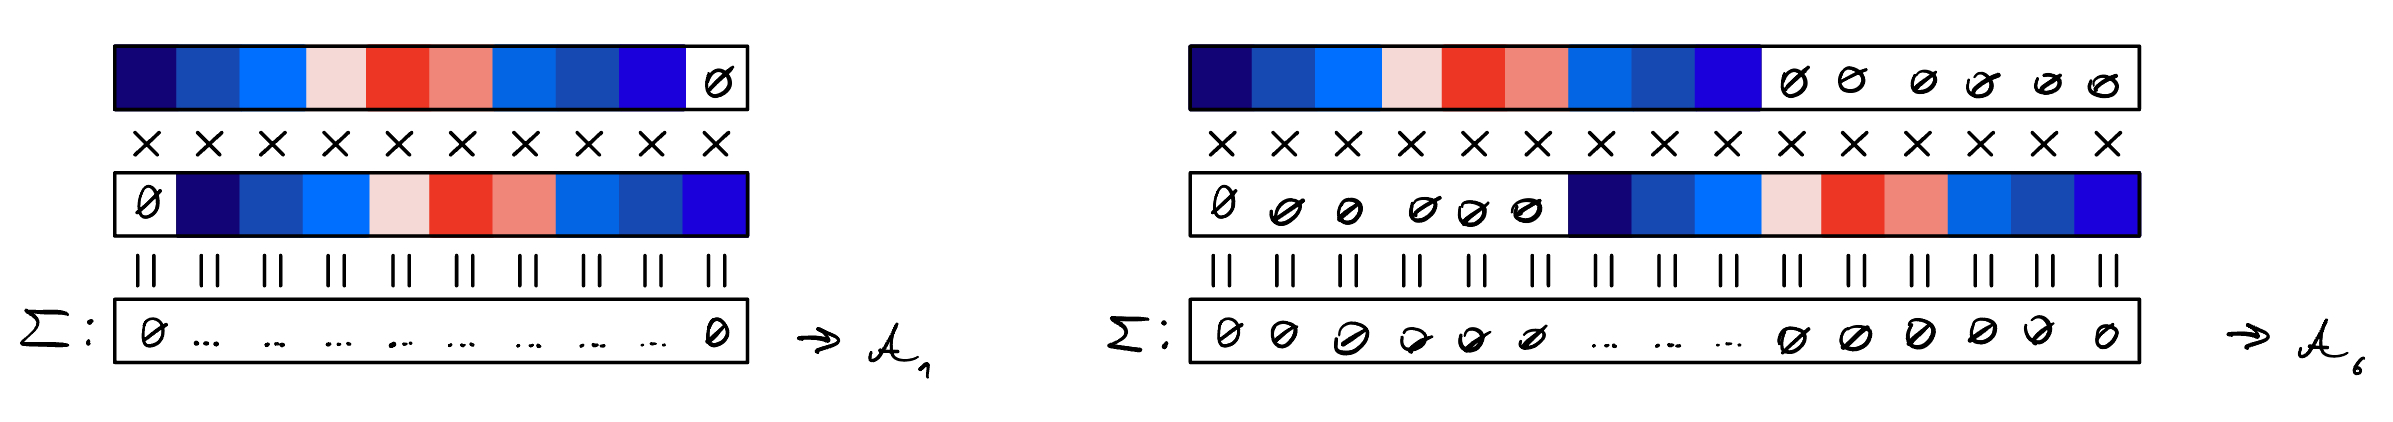
\includegraphics[width=0.9\textwidth]{figures/chap2/ACF_bound.jpeg}
    \caption{[TO IMPROVE] Schematic representiation of boundary effects when computing the autocorrelation function on the whole signal. Since the signal is finite, the contributions on the borders are set to zero.}
    \label{fig:ACF_bound}
\end{figure}
\begin{figure}[h!]
    \centering
    \includegraphics[width=0.5\textwidth]{figures/chap2/ACF_window.jpeg}
    \caption{[TO IMPROVE] Schematic representiation of windowed autocorrelation. In contrast to a full-width ACF, here no boundary effects arise.}
    \label{fig:ACF_window}
\end{figure}
It is then worth limiting the signal in a central window of length $2W$ and computing the ACF on the windowed signal (Fig.\ \ref{fig:ACF_window}). Taking as input the latter as $Z_0,\dots,Z_{2W-1}$, the output will be a series of values $\mathcal{A}_0,\dots,\mathcal{A}_{W}$ living in the space-domain\footnote{While the FFT domain is made of frequencies, the ACF domain is instead made of lag values, corresponding to the spatial shifts of the signal.} such that:
\begin{equation*}
    \mathcal{A}_k = \frac{1}{2} \left( \frac{\sum_{n} Z_n Z_{n+k}}{\sqrt{\sum_{n} Z_n^2 \sum_{n} Z_{n+k}^2}} + \frac{\sum_{n} Z_n Z_{n-k}}{\sqrt{\sum_{n} Z_n^2 \sum_{n} Z_{n-k}^2}} \right)\, .
\end{equation*}
This formula computes the windowed autocorrelation by shifting the signal both to the left and to the right and then taking the average.
Both terms are normalized in order to get $\mathcal{A}_0 = 1$. 
Note that the sums run from $n = 0$ to $n = W-1$ and thus the length of the signal must be greater than $4W$: data that does not respect this condition will not be analyzed.

The computation of this function on some simple signals is shown in App.\ \ref{chap:app_ACF}. In contrast to the FFT, the ACF results, as mentioned before, live in the space-domain and give direct results on the length scales. A high ACF value at $\Delta x_0$ means that the signal is correlated with itself when shifted by $\Delta x_0$. The periodicity of the signal is then related to the length $\Delta x_0$.

\subsection{FFT and ACF analysis on sequences}
Now, what we shall do is computing the FFT and the ACF on the data, taking care of the fact that it is necessary to separate the inside region (the bubble) from the outside one. This is done by relying on the piecewise exponential fit results, namely the positions $x_1$ and $x_2$ from Eq.\ \eqref{eq:fit_exp}.
\begin{figure}[h!]
    \centering
    \includegraphics[width=\textwidth]{figures/chap2/inside_omdet.png}
    \caption{Example of FFT and ACF calculated on the inside region of shots with $\Omega_R/2\pi = 400$ \unit{\hertz} and $\delta/2\pi = 596.5$, after selecting the shots where $x_2-x_1 > 4W = 80$. The values for each shot are shown in the left graphs with colormaps, while the averages on all shots are on the right. Note that before computing the transforms the data was set to zero-mean by subtracting its average. In the lower right graph, ACF computed on the true data (without the 0-mean) is shown for comparison to the other ACF profile.}
    \label{fig:inside_00}
\end{figure}
% We will also compute the transforms on the no-bubble shots. 
An example of the inside region analysis for a selected pair of values $\Omega_R, \delta$ (the same of Fig.\ \ref{fig:sorting}) is presented in Fig.\ \ref{fig:inside_00}, where the data was first set to zero-mean and only the shots where $x_2-x_1 > 4W$ are selected.
% One can probably (with a good eye) already see in the colormap plot that two or three vertical bands extend over all shots and appear at the same frequencies. This ensures that the FFT averaging is rightful.

Let us briefly discuss the behaviours of the computed FFTs and ACFs, considering that it is similar for all sequences and the example presented is a good one (see Fig.\ \ref{fig:inside_avg}, showing the profiles averaged over all sequences with the same $\Omega_R$). The FFT shows a peak at a frequency in the order of $k_{\rm FFT} \sim 0.01$ \unit{\per\micro\meter} and of width in the order of $\Delta k_{\rm FFT} \sim 0.1$ \unit{\per\micro\meter}. The ACF instead has a first peak at $\Delta x_{\rm ACF} \sim 10-11$ \unit{\micro\meter}. By comparing these results and relying on the FFT and ACF definitions, the relation should be $k \sim 1/\Delta x$. However, by taking the inverse of the ACF peak values, one gets $k_{\rm ACF} \sim 0.1$ \unit{\per\micro\meter}, a frequency hidden in the FFT plot due to the broad peak. The reason for the peak broadness is probability the data noise, which is difficult to analyze properly. We will thus proceed by relying only on the ACF for the remaining analysis.

\begin{figure}[t!]
    \centering
    \includegraphics[width=\textwidth]{figures/chap2/inside_fft_avg.png}
    \caption{FFT and ACF profiles (computed with zero-mean data) averaged over all sequences with the same radiation coupling $\Omega_R$. On the top, the FFTs are plotted both in the $k$-domain and $x$-domain. On the bottom, che ACFs are also plotted in the two domains to match the upper panel and confront the results.
    The FFTs are peaked at $k_{\rm FFT} \sim 0.01$ \unit{\per\micro\meter}, while the first ACF peaks are at $\Delta x_{\rm ACF} \sim 10-11$ \unit{\micro\meter}.}
    \label{fig:inside_avg}
\end{figure}

\subsection{ACF analysis on all shots}
From now on, all shots will be considered, taking into account all $\Omega_R$ and $\delta$ values. What we shall proceed to do is studying the ACF parameters as functions of the bubble properties, such as the experimental waiting time and the bubble size, and of the experimental external parameters: the coupling $\Omega_R$ and the detuning $\delta$. 
The routine is the following:
\begin{enumerate}
    \item Gather all shots with the same $\Omega_R$ and save their bubble parameters;
    \item Select only the shots where the inside or outside region is at least $4W$ pixels long;
    \item Sort the shots based on the waiting time or the bubble size;
    \item Cluster the shots based on the sorting parameter;
    \item Compute the ACF profile for each shot in a cluster and take the average;
    \item Plot the ACF averages for each cluster and fit them;
    \item Plot the fit results vs the time or size averages in each cluster.
\end{enumerate}
The number of analyzed inside and outside shots is shown in Tab.\ \ref{tab:shots}.
\begin{table}[h!]
    \centering
    \begin{tabular}{c|c|c|c}
        $\Omega_R/2\pi$ [\unit{\hertz}] & \# all shots & \# inside shots & \# outside shots \\
        \hline
        300 & 1491 & 1435 & 938\\   
        400 & 660 & 604 & 489\\
        600 & 718 & 561 & 717\\
        800 & 159 & 117 & 159\\     
    \end{tabular}
    \caption{Number of shots selected (where the inside or outside length is sufficient for the ACF computation). It is noticeable that the inside data for 300 \unit{\hertz} is way bigger than the rest.}
    \label{tab:shots}
\end{table}

\paragraph{Inside}
The ACF outside profiles can be fitted with a damped cosine of the form
\begin{equation*}
    \mathcal{A}_{\rm fit}(x) = (1 - \Delta)\cos(\frac{x}{\ell_2})\exp[-\left(\frac{x}{\ell_1}\right)^\alpha] + \Delta\, ,
\end{equation*}
with $\alpha = 1.7$ fine-tuned in order to capture the profile in the best way possible.\footnote{Literature suggests to use $\alpha = 2$, a gaussian damping.} One could theoretically set $\alpha$ as a fit parameter, but this would result in a worse estimation of the length $\ell_1$, with the fit that adapts to the data by changing only $\alpha$.

An example of fit on the inside shots is presented in Fig.\ \ref{fig:fit_time_inside}, where the shots are grouped by time. The parameters retrieved from the fit are in Fig.\ \ref{fig:param_time_inside} and \ref{fig:param_size_inside}. A global fit on all shots with the same radiation coupling is in Fig.\ \ref{fig:fit_omega_inside}.
\begin{figure}[h!]
    \centering
    \includegraphics[width = \textwidth]{figures/chap2/fit_size_inside.png}
    \caption{ACF average profiles of inside shots grouped by size in 10 blocks (solid lines) and fitted with the damped cosine (dotted lines) for each value of $\Omega_R$. Size increases from darker to lighter colors.}
    \label{fig:fit_time_inside}
\end{figure}
\begin{figure}[h!]
    \centering
    \includegraphics[width = \textwidth]{figures/chap2/param_size_inside.png}
    \caption{Fit parameters $\ell_1$, $\Delta$ and $\ell_2$ of inside shots grouped by size (in log scale).}
    \label{fig:param_size_inside}
\end{figure}
\begin{figure}[h!]
    \centering
    \includegraphics[width = \textwidth]{figures/chap2/param_time_inside.png}
    \caption{Fit parameters $\ell_1$, $\Delta$ and $\ell_2$ of inside shots grouped by time (in log scale).}
    \label{fig:param_time_inside}
\end{figure}
\begin{figure}[h!]
    \centering
    \includegraphics[width = \textwidth]{figures/chap2/fit_omega_inside.png}
    \caption{ACF average profiles of inside shots grouped by $\Omega_R$ (solid lines) and fitted with the damped cosine (dotted lines).}
    \label{fig:fit_omega_inside}
\end{figure}
The time dependence seems to be the most noticeable. From Fig.\ \ref{fig:param_time_inside}, the first parameter $\ell_1$ is decreasing with time, while the second parameter $\Delta$ is increasing and approaching 1. This behaviour could mean that the magnetization inside the bubble loses (?) its spatial information with time.

\paragraph{Outside}
On the other hand, for the outside region ACF fit we use an exponential
\begin{equation*}
    \mathcal{A}_{\rm fit}(x) = (1-\Delta)\exp[-\frac{x}{\ell_1}] + \Delta\, .
\end{equation*}
An example of fit on the outside shots is presented in Fig.\ \ref{fig:fit_time_outside}, where the shots are grouped by time. The parameters retrieved from the fit are in Fig.\ \ref{fig:param_time_outside}, \ref{fig:param_size_outside}. A global fit on all shots with the same radiation coupling is in Fig.\ \ref{fig:fit_omega_outside}.
\begin{figure}[h!]
    \centering
    \includegraphics[width = \textwidth]{figures/chap2/fit_size_outside.png}
    \caption{ACF average profiles of outside shots grouped by size in 10 blocks (solid lines) and fitted with the exponential (dotted lines) for each value of $\Omega_R$. Size increases from darker to lighter colors.}
    \label{fig:fit_time_outside}
\end{figure}
\begin{figure}[h!]
    \centering
    \includegraphics[width = \textwidth]{figures/chap2/param_size_outside.png}
    \caption{Fit parameters $\ell_1$ and $\Delta$ of outside shots grouped by size.}
    \label{fig:param_size_outside}
\end{figure}
\begin{figure}[h!]
    \centering
    \includegraphics[width = \textwidth]{figures/chap2/param_time_outside.png}
    \caption{Fit parameters $\ell_1$ and $\Delta$ and of outside shots grouped by time (in log scale).}
    \label{fig:param_time_outside}
\end{figure}
\begin{figure}[h!]
    \centering
    \includegraphics[width = \textwidth]{figures/chap2/fit_omega_outside.png}
    \caption{ACF average profiles of outside shots grouped by $\Omega_R$ (solid lines) and fitted with the exponential (dotted lines).}
    \label{fig:fit_omega_outside}
\end{figure}
In contrast to the inside bubble region, what emerges outside the bubble is that the characteristic length of the autocorrelation $\ell_1$ is increasing with time and the offset is decreasing (Fig.\ \ref{fig:param_time_outside}), which is the opposite behaviour.

% \subsection{Border alignment}
